\chapter{Background}\label{ch:background}

First, we will need to explore the various types of CPU profiling commonly in use today, in particular statistical profiling, and familiarise ourselves with the available hardware support for performance monitoring. Then, we will begin to look at how the modern profiler on Linux, \texttt{perf} is implemented.

\section{Profiling}

We profile a program or system to gain a deeper insight into its runtime behaviour, often in response to a performance issue. The systems we may want to profile can range from hardware, operating systems, networks, cloud infrastructure, etc. Profiling differs from debugging, in that often we debug a program or system whenever it does not meet its functional requirements, compared to non-functional requirements.

\subsection{CPU Profiling}

In software systems, a large class of performance issues come down to understanding how and where execution time is being spent on the Central Processing Unit (CPU). Without that insight, it can be quite difficult to diagnose exactly where in the program the performance bottlenecks lie.

An example of a CPU profiler that has long been available on UNIX systems (in the case of BSD, since 1983 \cite{ManGprof}) is \texttt{gprof}.

\subsection{Types of CPU Profilers}\label{sect:cpu_profiler_types}

CPU profiling is an umbrella term which encompasses a number of different types and approaches. However, there are three prominent types and techniques used to collect timing data that we should consider when determining which approaches are most applicable in the context of seL4.

\subsubsection{Instrumentation}

Instrumentation is a profiling technique where trace functions are executed at the start (prologue) and end (epilogue) of each function call. The trace functions are able to collect precise timings during each call, creating a detailed summary of how much time was spent in each function in the program.

With GCC for example, the \texttt{-pg} flag will generate trace functions that automatically collect timing information, which by default, is written to a file called gmon.out. The tool \texttt{gprof} can then be used to view the data. Alternatively, user defined trace functions can be called instead via the GCC flag \texttt{-finstrument-functions} \cite{ManGCC}. 

\subsubsection{Statistical}\label{sect:statistical}

Statistical profiling involves sampling the program counter and call stack running on the CPU at regular intervals. It differs from instrumentation, in that it does not provide a complete picture of the program's execution, but rather an estimation. The trade-off is that statistical profiling allows the program to run closer to full speed, since the cost to profile is not incurred during each function call. We will discuss the mechanics of statistical profiling at greater length in Section \ref{sect:statistical_profiling}.

\subsubsection{Event-based}

Both instrumentation and statistical profiling are mainly concerned with capturing timing information, such that execution time on the CPU can be attributed to functions within the program. Undoubtedly, this is a valuable tool when trying to quickly understand where in the program an unexpected amount of time is being spent. However, not all performance issues can be resolved in software alone, but rather require greater insight into the microarchitectural events occurring within the CPU to understand the complete picture. These architectural events may be branch misses, cache misses, context switches, TLB misses, page faults etc.

\subsection{Statistical Profiling Overview}\label{sect:statistical_profiling}

\subsubsection{Code Execution}

In this discussion on code execution, we refer to a thread as the basic unit of CPU utilisation, which consists of a program counter (PC), a call stack, and a register set. The PC is a register on the CPU that stores the address of the instruction currently being executed\footnote{For processors that implement instruction pipelining, when an instruction is in the execution stage (EX), the PC typically will no longer refer to that particular instruction, but rather the instruction in the instruction-fetch (IF) stage of the pipeline.}. The call stack is a data structure, typically resident in Random Access Memory (RAM), that keeps track of the nested function calls, and stores the required state for each function (such as local variables). The register set refers to the current value within each register on the CPU (known as a \textit{core} register). 

\subsubsection{Sampling}

Following from the brief overview of statistical profiling in \ref{sect:statistical}, a statistical profiler will sample the PC at each interval. Over time, a number of samples will be collected, which can then be processed to generate an execution profile. 

\begin{figure}[!h]
    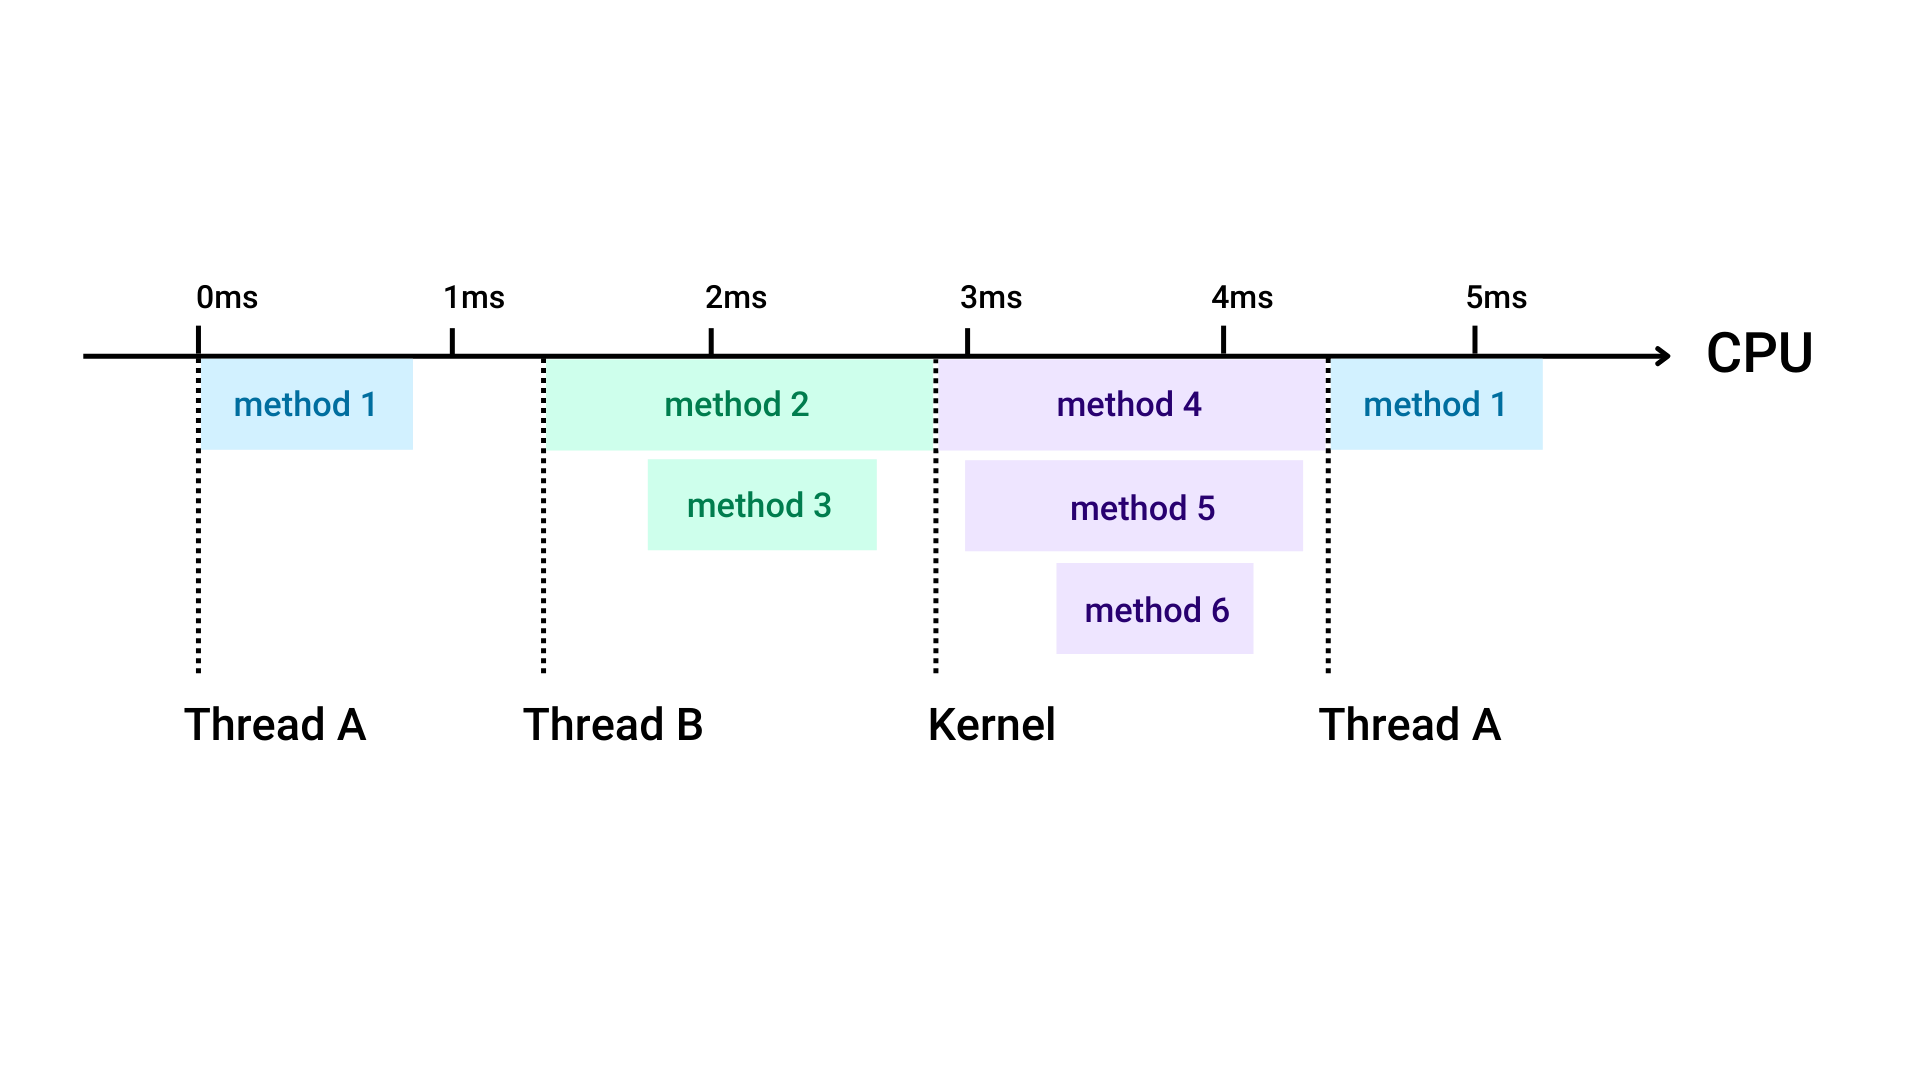
\includegraphics[width=\linewidth]{report-a_sampling_timeline}
    \caption{Sampling the CPU every 1ms. In this example, profiling begins at 0ms, where the first sample is recorded with thread A on the CPU executing method 1. The second sample occurs at 1ms, where there is no activity on the CPU. At 2ms, thread B is active and the call stack contains methods 2 and 3. The fourth sample at 3ms, records only method 4 executing within the kernel. This example was adapted from the one presented at the Dotnetos conference talk ``CPU profiling inside out" \cite{YouTubeDotnetosCPUProfling}.}
    \label{fig:sel4_microkernel}
\end{figure}

A statistical profiler needs to employ some mechanism in order to probe the CPU state at regular intervals. This is referred to as the \textit{profiling interrupt}. In the case of \texttt{gprof}, initially on Linux (v2.0 and earlier) it used the syscall {\texttt{setitimer} \cite{DocsGProfImpl}, which permitted it access to the underlying hardware timers. Then later it migrated to the more efficient \texttt{profil} syscall where the kernel could perform the probe on behalf of the user program, and therefore did not require two mode switches when the timer interrupt occurred. While hardware timers are still extensively used in modern processors, there is now dedicated hardware for performance profiling, which is covered at depth in Section \ref{sect:pmu}.

\section{Performance Monitoring}

\subsection{Microarchitecture}

The Instruction Set Architecture (ISA) is the interface between software and hardware. It is part of the abstract model of a computer, and defines how the CPU is controlled by software \cite{GlossArmISA}. The term microarchitecture refers to how a given ISA is implemented in a particular processor. A processor (CPU) consists of a number of components with different responsibilities, that harmoniously coordinate to execute each instruction. To help illustrate how these components fit together, Figure \ref{fig:cpu_vis} shows a hypothetical processor, where the RAM and system clock are not part of the CPU, but rather shared with the rest of the system.

\begin{figure}[!ht]
    \centering
    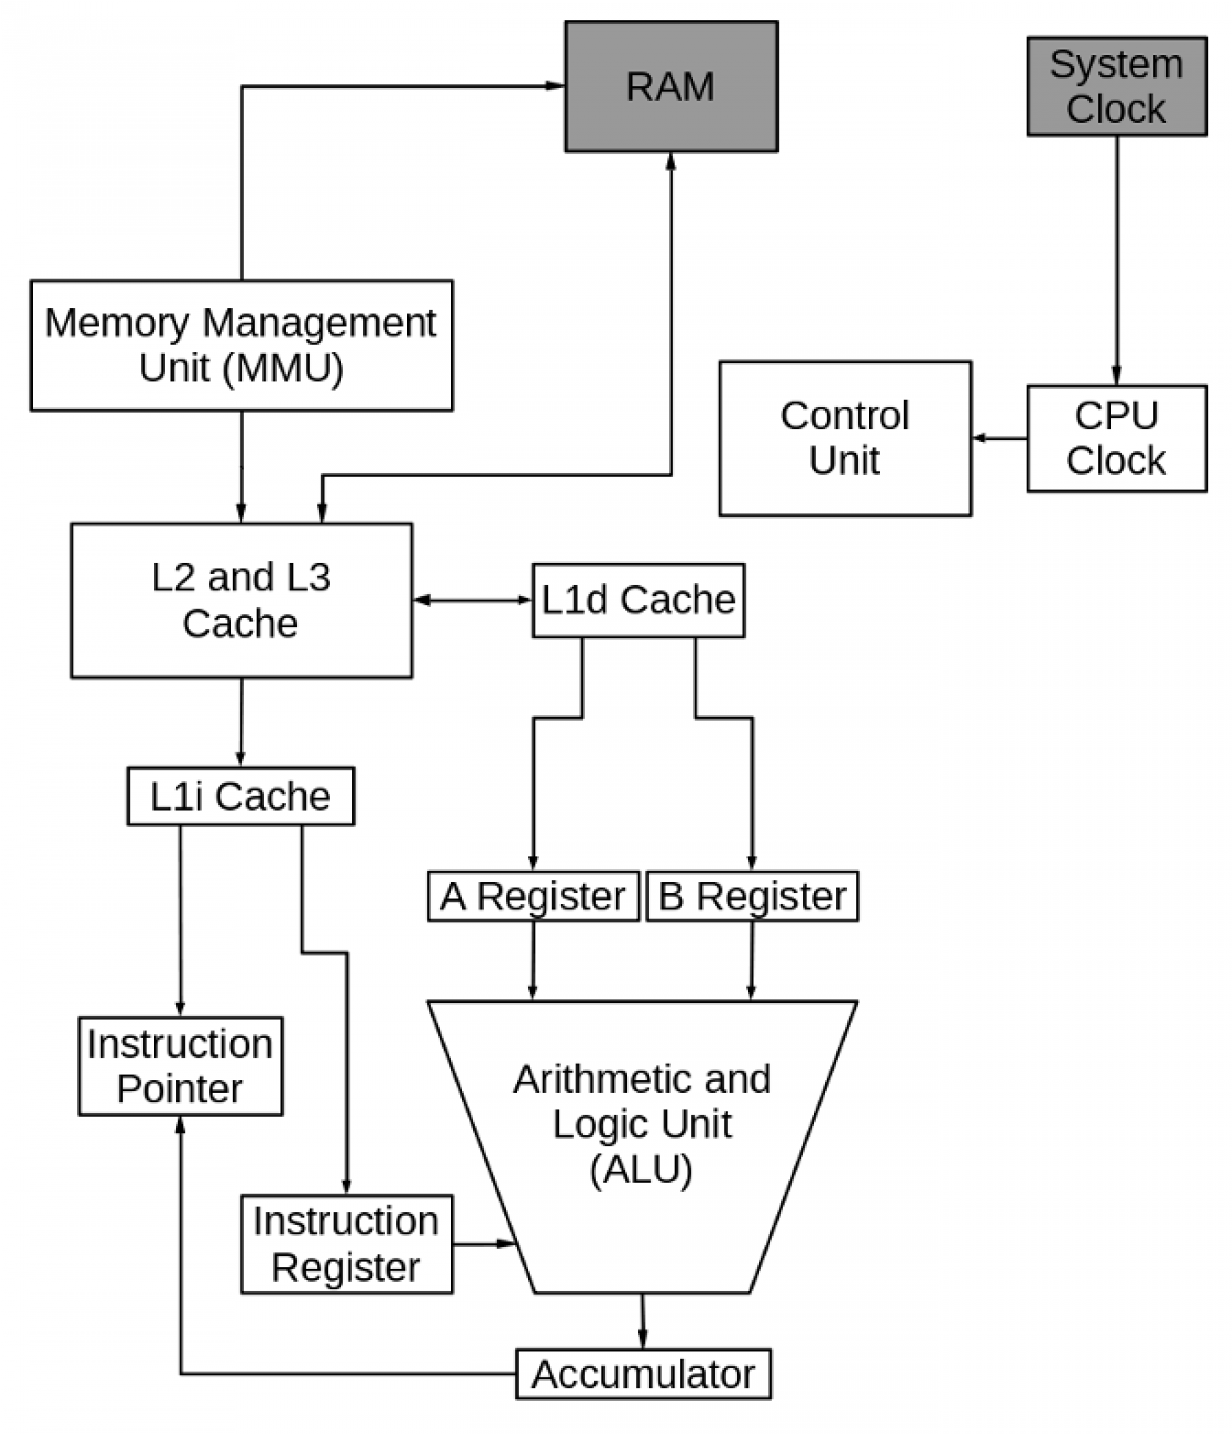
\includegraphics[width=0.5\linewidth]{redhat_cpu_vis}
    \caption{A simplified conceptual diagram of a typical CPU. The reality is much more complex than this, however a typical CPU will have: multiple layers of caching (L1, L2, etc), distinct L1 cache for instructions (L1i) and memory (L1d), a Memory Management Unit (MMU) to support virtual addressing, a control unit to coordinate the data-path and pipelining, and an Arithmetic Logic Unit (ALU) to execute arithmetic and logical instructions. Taken from a Red Hat blog post titled ``The central processing unit (CPU): Its components and functionality" \cite{BlogRedHatCPU} } 
    \label{fig:cpu_vis}
\end{figure}

\subsection{Performance Monitoring Unit (PMU)}\label{sect:pmu}

A statistical profiler can help determine where in the program an unexpected amount of time is being spent, but unless the root cause is solely in software, it is not able to provide any insight into where time is being spent within the microarchitecture itself.

The Performance Monitoring Unit (PMU) is a non-invasive debug component, which can addresses this limitation, by providing a fixed number of counters that can count various useful events that regularly occur with the CPU itself. Note, while the PMU provides greater capabilities for software based profilers, it is also used by hardware engineers to debug potential hardware issues and perform microarchitecture benchmarks.

\subsubsection{Hardware Events}

The events available to be counted on the PMU vary from processor architecture (e.g x86 vs ARM), but they also can vary between processors within the same architecture (e.g Cortex-M55 vs Cortex-M33). However PMU events can be typically grouped into the following event type categories \cite{DocsArmv8PMU}:

\begin{multicols}{2}
\ssp
\begin{itemize}
    \item Instruction execution
    \item Instruction speculation
    \item Cache behaviour 
    \item External memory accesses
    \item Memory errors
\end{itemize}
\columnbreak
\begin{itemize}
    \item Branch prediction
    \item Exceptions
    \item Pipeline stalls
    \item CPU cycles
    \item Debug and trace events
\end{itemize}
\dsp
\end{multicols}

\subsection{Performance Counters}

At a high level, the PMU allows a single, supported event to be assigned to one of the available performance counters. Commonly, the PMU can be interfaced via Model Specific Registers (MSRs), which are a set of registers on the processor\footnote{Typically the registers are not located on the CPU itself, but rather on a coprocessor. This decouples the PMU from the main processor since on most architectures the PMU is an optional extension.} that dictate how the PMU should operate.

\subsubsection{Fixed and Programmable Counters}

In practice, most PMUs offer a mix of both fixed and programmable counters. Fixed performance counters always count the same event within the CPU. They are used for common used events, such as CPU cycles and instructions retired. Programmable counters, as the name suggests, can be programmed to count any supported\footnote{On x86, some events can only assigned to a subset of the available performance counters, and therefore are considered semi-programmable. In order to determine which events can be assigned to which counters, x86 provides a mask for each event which specifies the supported counters.} event.

\subsection{Counting vs Sampling}\label{sect:sampling_counting}

Generally, there are two distinct use cases when wanting to utilise the PMU. The first, known as \textit{counting}, is when we want to record the number of times a particular event has occurred whilst a specific operation was executing. To do so, we reset the value of the counter to 0, perform the operation, and then read the value of the counter again. 

The second use case, known as \textit{sampling}, is when we want the PMU to notify us once the count for a certain event reaches a particular value. When this occurs, known as a counter \textit{overflow}, the PMU signals an interrupt informing us that the overflow has occurred. 

\subsection{Programming the PMU}\label{sect:programming_pmu}

To help illustrate how to interface with the PMU, we will demonstrate how to program the PMU to count the number of instruction software increments on an ARMv7-A processor that uses the Performance Monitors Extension version 2 (PMUv2). Instruction software increments refers to when the instruction has been architecturally executed. This will differ from the number of CPU clock cycles, since a given instruction may take multiple CPU cycles to execute. This event is also known as \textit{instruction retired} on other platforms.

\subsubsection{Cortex-A15}

The Cortex-A15 is a 32-bit multi-core processor, which implements the ARMv7-A architecture, and is well supported by seL4 \cite{DocsSeL4Hardware}. The PMU on the Cortex-A15 implements the PMUv2 architecture and provides six programmable counters \cite{DocsArmCortexA15PMU} and one clock cycle counter (PMCCNTR). The ARMv7-A architecture defines 12 performance monitor registers (PMRs) which are used to configure the behaviour of the PMU \cite{DocsArmv7PMURegs}. The PMU registers reside on Coprocessor 15 (CP15). For this example, adapted from the Resource Allocation and Scheduling Group \cite{TutHowToUsePMU}, only the following six registers are required:

\ssp

\begin{itemize}
    \item Performance Monitor Control Register (PMCR)
    \item Count Enable Set Register (PMCNTENSET)
    \item Overflow Flag Status Register (PMOVSR)
    \item Event Count Selection Register (PMSELR)
    \item Event Type Select Register (PMXEVTYPER)
    \item Event Count Register (PMXEVCNTR)
\end{itemize}

\dsp

To begin, we will define a series of \#defines to provide greater clarity regarding the value being written to a particular PMU register (defined in Listing \ref{lst:pmu_flags}). Note, the constants are directly from each respective PMU register section in the ARM Architecture Reference Manual ARMv7-A and ARMv7-R edition \cite{DocsArvm7}.

\begin{listing}[!ht]
    \begin{minted}{C}
#define PMU_SOFTWARE_INC_EVT_ID         0x00

#define PMCR_EN_CTRS                   (0x1 << 0)
#define PMCR_EN_RESET_CTRS             (0x1 << 1)
#define PMCR_EN_RESET_CLK_CTR          (0x1 << 2)
#define PMCR_EN_CLK_DIV                (0x1 << 3)
#define PMCR_EN_EXPORT_EVTS            (0x1 << 4)
#define PMCR_DD_CLK_CTR_PROB_REG       (0x1 << 5)

#define PMCNTENSET_EN_PMCCNTR          (0x1 << 31)
#define PMCNTENSET_EN_CTRS              0x3F

#define PMOVSR_EN_PMCCNTR              (0x1 << 31)
#define PMOVSR_EN_CTRS                  0x3F
    \end{minted}
    \caption{Flags for PMU MSRs on ARMv7.}
    \label{lst:pmu_flags}
\end{listing}

\subsubsection{Initialising the PMU}

When the processor is first powered on, we have to assume that the PMU registers are in an undefined state and therefore reinitialise them. This involves enabling counters, resetting them to 0, as well as the clock counter. To write to one of the PMU registers on ARMv7, we use the Move to Coprocessor (MCR) instruction \cite{DocsArmMCR} (Listing \ref{lst:pmu_pmcr}). Often, we want to use performance counters within a C program, and therefore we are using inline assembly, in particular Extended Asm \cite{DocsGCCExtendedAsm}.

\begin{listing}[!ht]
    \begin{minted}{C}
uint32_t pmcr_config = PMCR_EN_CTRS
                     | PMCR_EN_RESET_CTRS
                     | PMCR_EN_RESET_CLK_CTR;
asm volatile ("MCR p15, 0, %0, c9, c12, 0\t\n" :: "r"(pmrc_config));
    \end{minted}
    \caption{Initialising the counters via the \texttt{PMCR}.}
    \label{lst:pmu_pmcr}
\end{listing}

Now that counters are initialised, we need to enable the specific counters that we want to use. In this case, we will enable counter 0, as well as the clock counter (Listing \ref{lst:pmu_pmcntenset}).

\begin{listing}[!ht]
    \begin{minted}{C}
uint32_t pmcntenset_config = PMCNTENSET_EN_CTRS | PMCNTENSET_EN_PMCCNTR;
asm volatile ("MCR p15, 0, %0, c9, c12, 1\t\n" :: "r"(pmcntenset_config));
    \end{minted}
    \caption{Enabling counter 0 and the CPU clock counter via the \texttt{PMCNTENSET} register.}
    \label{lst:pmu_pmcntenset}
\end{listing}

Finally, we need to clear the overflow bit for both of the counters (Listing \ref{lst:pmu_pmovsr}).

\begin{listing}[!ht]
    \begin{minted}{C}
uint32_t pmovsr_config = PMOVSR_EN_CTRS | PMOVSR_EN_PMCCNTR;
asm volatile ("MCR p15, 0, %0, c9, c12, 3\t\n" :: "r"(pmovsr_config));
    \end{minted}
    \caption{Clearing the overflow bit (in case it was previously enabled) via the \texttt{PMOVSR}.}
    \label{lst:pmu_pmovsr}
\end{listing}

\subsubsection{Counting an event on the PMU}

Once we have initialised the PMU, we can assign the software increment event to counter 0. This is a two step process. First we specify which counter via \texttt{PMSELR}, and then we specify which event via \texttt{PMXEVTYPER} (Listing \ref{lst:pmu_assign_ctr}).

\begin{listing}[!ht]
    \begin{minted}{C}
asm volatile ("MCR p15, 0, %0, C9, C12, 5" :: "r"(0x00));
asm volatile ("MCR p15, 0, %0, C9, C13, 1" :: "r"(PMU_SOFTWARE_INC_EVT_ID));
    \end{minted}
    \caption{Assigning the software increment event to counter 0 via \texttt{PMSELR} and \texttt{PMXEVTYPER}.} 
    \label{lst:pmu_assign_ctr}
\end{listing}

\subsubsection{Reading an event count on the PMU}

The PMU will begin to count the number of software increment events as the program continues to execute on the CPU. At any stage, the current count can be obtained from the PMU register \texttt{PMXEVCNTR}. In this case, we use the Move to ARM Register \cite{DocsArmMRC} instruction to move the value from a Coprocessor register to a core (CPU) register, which will be written into the variable \texttt{counter\_value} (Listing \ref{lst:pmu_read_ctr}).

\begin{listing}[!ht]
    \begin{minted}{C}
uint32_t counter_value;
asm volatile ("MCR p15, 0, %0, C9, C12, 5" :: "r"(config.counter));
asm volatile ("MRC p15, 0, %0, C9, C13, 2" : "=r"(counter_value));
    \end{minted}
    \caption{Reading the number of software increments in counter 0 via the PMXEVCNTR.} 
    \label{lst:pmu_read_ctr}
\end{listing}

\section{Platform Support}\label{sect:platform_support}

\subsection{x86 Systems}

x86 systems are ubiquitous in desktop computing, workstations, and servers. A majority of CPUs in the TOP500 project are based on x86-64 \cite{SiteTop500Project}. The x86-64 architecture is the 64-bit version of the x86 ISA. The x86 ISA is a Complex Instruction Set Architecture (CISC), which tend to have higher power requirements, but in return offer higher performance over RISC architectures for certain kinds of workloads, such as vector operations since x86 supports Single Instruction, Multiple-Data (SIMD) instructions. Both Intel and AMD produce processors that implement the x86 ISA.

Performance monitoring was first introduced in the Intel Pentium processor with a set of model specific performance monitoring counter MSRs. Intel refers to its x86 (32-bit) and x86-64 architecture implementations as Intel 64 and IA-32 respectively. There are two classes of performance monitoring capabilities offered by the Intel architectures \cite{DocsIntel64IA32Vol3B}:
\begin{itemize}
    \item \textit{architectural} - visible behaviour of events are consistent across processor implementations.
    \item \textit{non-architectural} - events are specific to the microarchitecture and vary from processor to processor.
\end{itemize}

The number of general-purpose performance monitoring counters can vary across processor generations within a processor family, across processor families, or could be different depending on the configuration chosen at boot time in the BIOS regarding Intel Hyper Threading Technology. Typically there are between 2-8 programmable performance counters, and three fixed counters.

\subsection{ARM Systems}

The ARM processors are frequently utilised in embedded systems, due to their low cost, minimal power consumption and lower heat generation compared to their competitors \cite{ArticleEmbeddedTwoPercSol}.

The ARM processor family is divided into three architecture profiles \cite{DocsArmArchProfiles}:
\begin{itemize}
    \item Application (\textit{A-profile}): Highest performance, targeted towards operating systems. The distinguishing feature from the other two profiles is that supports virtual memory via a Memory Management Unit (MMU).
    \item Real-time (\textit{R-profile}): Fast response, targeted towards high-performance, hard real-time applications.
    \item Microcontroller (\textit{M-profile}): Lowest power consumption, targeted towards microcontrollers and discrete processing. It is designed to be integrated into an FPGA.
\end{itemize}

The ARMv8 architecture (most recent is ARMv9, announced March 2021) supports up to 31 programmable performance counters, however in practice, processors that implement the ARMv8 architecture only provide between 4-8 counters \cite{DocsArmCortexR52PMUCtrs} \cite{DocsArmCortexM55PMUCtrs}.

\subsection{RISC-V Systems}

RISC-V is royalty free, open-source ISA and processor specification for a Reduced Instruction Set Computer (RISC) architecture. Historically, RISC-V was prominently used in academia, since researches are able to change and experiment with the architecture. However, in recent years, there has been a sharp rise in the commerical viability of RISC-V processors, replacing systems that were traditionally dominated by ARM \cite{BlogVentureBeat}.

The RISC-V ISA specification defines three fixed performance counters (\texttt{hpmcounter0} to \texttt{hpmcounter2}) which are dedicated for cycle count, real-time clock and instructions-retired respectively. It also supports up to 29 programmable performance counters (\texttt{hpmcounter3}-\texttt{hpmcounter31}) \cite{DocsRISVISAPerfCounters}.